The \textit{singularity} is a term first coined by Vernon Vinge and popularized, 
later on, by Ray Kurzweil in a series of books published by early 2000's.
\cite{age, singularity} 

It refers to a point in technologial progress (particularly in the field of 
Artificial Intelligence) where \textbf{machine's capabilities will overcome all human 
intelligence combined.}

Vinge's article hesitates to asses singularity's feasibility (He isn't 100\% sure 
but "If it can happen, It will", he concedes), Kurzweil stance is significatively 
more bold: \textit{he actually made predictions.}\footnote{
	It is relevant noticing that Mr. Kurzweil, Google's director of engineering, 
	is a reputated futurist. Thus, we can see the predictions listed above as a 
	curated summary on Artificial Intelligence's \textit{state of the buzz}
}

Regarding artificial intelligence, the steps that will pave the road to the 
singularity are\cite{interview}: 

\begin{itemize}
	\item [\textbf{\textcolor{secondary}{2009}}] Speech-to-speech automated 
		translation will be available in cell phones.

	\item [\textbf{\textcolor{secondary}{2017}}] Computers will be ubiquitous, 
		smaller, integrated in our clothes and some of them sel-organized.

	\item [\textbf{\textcolor{secondary}{2017}}] Full inmersive virtual reality 
		will be available.
	
	\item [\textbf{\textcolor{secondary}{2018}}] 10TB of memory storage (roughly 
		the human brain capacity) will cost less than \$1000.

	\item [\textbf{\textcolor{secondary}{2020}}] A computer is expected to pass 
		Türing's test. 

	\item [\textbf{\textcolor{secondary}{2023}}] $10^{16}$ calculations per second 
		will be possible in a cheap machine.

	\item [\textbf{\textcolor{secondary}{2029}}] Computers will have achieved 
		human-level intelligence.

	\item [\textbf{\textcolor{secondary}{2025}}] Military-grade UAV's will be 
		100\% autonomous.

	\item [\textbf{\textcolor{secondary}{2045}}] \textbf{Singularity}. Artificial 
		Intelligences will became the smartest and most skilled creatures in earth.

\end{itemize}

Kurzweil's confidence is built on top of \textit{"The law of accelerated returns"}, \cite{law}, 
which states that: 

\vspace{.5cm}
\textcolor{gray}{
	\textit {
		\Large {
			"Rate of progress of an evolutionary process increases exponentially 
			[and] technology is such another evolutionary progress"
		}
	}
}
\vspace{.5cm}

Reallity seems to follow Kurzweil's predictions: it is possible to buy a 10TB 
Seagate Barracuda for $\sim400$\euro{}, Virtual (or augmented) reality systems 
have become popular in the last few years, Machine's translation has seen 
spectacular\footnote{
	It's not only Google Translate new arquitecture, it worth to mention Waverly Labs's 
	earphones\cite{pilot}, a new gadget that promises live and wearable machine translation.
} advances... 

And inspite of, in practice, every exponential growth is exponential until is not,
Microprocesors industry have conformed Moore's Law (an equivalent formulation of 
the same principle) for decades.

But most of machine learning's whispering are built on top of modern neural network
capabilities. After the publication of backpropagation \cite{back} algorithm, and the rise 
of cloud computing, neural network applications have grown rapidly. Nowadays, 
finding impressive examples of neural networks adopting nearly-human behaviours 
is susrprisingly easy: 

\begin{itemize}
	\item They can \textit{dream}.\cite{dream}
	\item They describe pictures.\cite{caption}
	\item They can code a website by their own.\cite{code}
	\item They are playing video games.\cite{snake}
\end{itemize}

	\begin{figure}[h!]
\begin{center}
		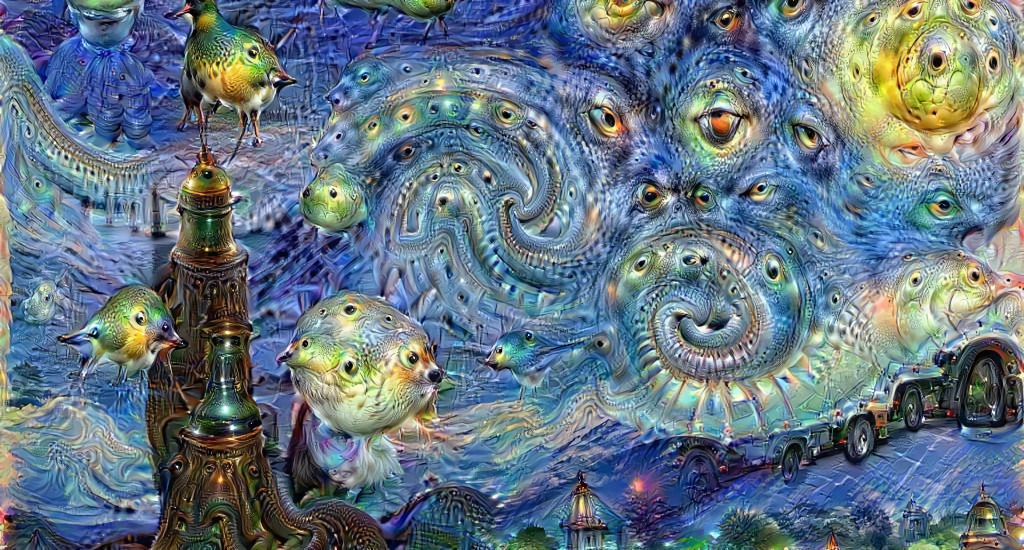
\includegraphics[width=\linewidth]{images/dream.jpg} % Figure image
		\caption{A neural network dreaming} % Figure caption
		\label{dream} % Label for referencing with \ref{bear}
\end{center}
	\end{figure}

The temptation to attribute human behaviour to AI systems is stronger today than 
it ever was. Therefore it looks that we should agree Mr Kurzweil: the singularity 
is near. 

Is it?